\documentclass[12pt]{article}
\usepackage[latin1]{inputenc}
\usepackage[T1]{fontenc}
\usepackage{lmodern}  
\usepackage{amsmath}
\usepackage{amsfonts}
\usepackage{amssymb}
\usepackage{mathtools}
\usepackage{geometry} 
\usepackage[round]{natbib} 
\usepackage{array}
\usepackage{multirow}
\usepackage{subfig}   
\usepackage[english]{babel}
\usepackage{graphicx} 
\usepackage{fancyhdr}
\pagestyle{fancy}
\fancyhf{}
\rfoot{\thepage}
\renewcommand\headrulewidth{0 pt}
\usepackage{lineno}
\geometry{tmargin=2.5 cm, bmargin=2 cm}

\captionsetup{labelfont=bf}  
\newcommand\equa[1]{\frac{\mathrm{d}#1}{\mathrm{d}t}}
\newcommand\barre[1]{\overline{\rule{0pt}{1.5ex}#1}}
\newcommand\unite[1]{\;\mathrm{#1/kg^{0.75}/day}}
\newcolumntype{M}{>$ c <$}
\newcommand\tit[1]{\multicolumn{1}{c|}{#1}} 
\linenumbers
\modulolinenumbers[2]
\bibliographystyle{AmNat}

\usepackage{color}

\begin{document}
\section*{Abstract}
Interspecific competition plays an important role in structuring communities but few studies have been done on herbivores. We present a competition model that predicts the outcome of competition between herbivore species competing for plants. Our model imbeds well-known concepts of the resource-ratio theory, such as the minimum level of resources, consumption vectors, and the quotas of resources required in the biomass. However, unlike traditional approaches that focused on plants as resources, we suggest that chemical elements and energy bounded in plant biomass represent the ultimate resources that herbivores compete for. Our model shows that the outcomes of competition between herbivores result from two main processes: the minimal requirement of resource for herbivores ($R^*$), and spatial segregation of resources embedded into different plants. The first process (minimal requirement) follows the classical $R^*$ rule and determines the competitive exclusion principle. On the other hand, foraging strategy of herbivores can allow coexistence because resources are spatially segregated. Put together, these two processes determine how herbivore species can coexist, since resources are bounded. Hence, a plant community rich in one resource should support an herbivore community rich in the same resource, leading to a bottom-up effect. 

\section*{Keywords}
competition, herbivore, chemical elements, resource ratio, ecological stoichiometry 

\section*{Introduction}
Interspecific competition for resources is thought to play an important role in structuring communities \citep{Gause1934,Tilman1987}. Modelling approaches have proven helpful to predict competitive outcomes, when resources are well identified and the number of different resources is limited. Hence, the theory is particularly well suited for autotrophic organisms (e.g., algae or plants) competing for essential nutrients \citep{Tilman1982}. Indeed, nutrients (i.e., chemical elements constituting biomass) are well-identified non-substitutable resources, and usually, competition is acute for only a few limiting nutrients, such as phosphorous (P), nitrogen (N), or potassium (K). In short, models  predict that niche  segregation  along  resource ratios should promote species coexistence. For example,  plants with low N:P requirement are more likely to coexist  with plants with high N:P requirement. \cite{Tilman1980} provided a graphical representation  based on Zero-Net-Growth Isoclines and consumption vectors, usually referred  to as the resource-ratio theory. In the last few decades, the resource-ratio theory has helped  popularize the use of competition models to predict competitive outcomes in experimental set ups and in  semi-natural conditions.\par 
However, the transfer of such a theory to higher trophic levels is not obvious. The main reason is that for heterotrophic organisms, resources are not easy to characterize. Consider for instance the case of herbivores. %In many cases, plants are considered as resources, but this approach is problematic for, at least, two reasons. First of all, some challenging questions remain. 
If one considers that plant species are the resources herbivores compete for, questions arises: to what extent does a given herbivore require more of a given plant species than another? Should plant species be considered essential non-substitutable resources, or  substitutable resources? %These challenges are uneasy to tackle. The second reason is the important number of plant species that an herbivore can feed on. 
For example, the diet of the red deer (\textit{Cervus elaphus}) in Europe includes 145 different plant species \citep{Gebert2001}. As a consequence, predicting  competitive outcomes  in  heterotrophic communities with simple models remains challenging and limited to specific cases \citep{Murray2008}. This limitation may prevent significant progress in our understanding of community structure at higher trophic levels. \par 
We argue that if, on the other hand, one considers that nutrients and energy contained in plant biomass represent the resources, most of the upper-cited challenges disappear. Indeed, nutrients and energy  clearly are essential non-substitutable resources for heterotrophs. For example, nitrogen is required in proteins and nucleic acids, and phosphorous is required in phospholipids, nucleic acids, or bones. The number of essential nutrients required for heterotrophic organism biomass of heterotrophs does not exceed 26 \citep{sterner2002}. The fact herbivore's growth rate may be limited by food quality (e.g., the level of nitrogen or phosphorus in plant biomass) rather than food quantity has been widely documented \citep{Sterner1992, Hessen1992, Urabe1992}. Moreover, it is possible  to determine the requirements of a given herbivore for a given element, using metabolism studies \citep{Mould1981}. In addition, it is clear that the ratios of nutrients required in the biomass vary across herbivore species. For example, the C:N:P ratio markedly varies among zooplanktonic herbivores \citep{Andersen1991, Sterner1992}. %Cladocerans may be limited by nitrogen or phosphorus, at least during part of the year \citep{Urabe1992}. There is an influence on consumer growth by food quality \citep{Huxel1999}. Then, a relation between sestonic elements stoichiometry and specific component of zooplankton community can be observed \citep{Hassett1997}. This kind of interspecific variations is also observed for terrestrial species (see table \ref{besoins}). 
In table \ref{besoins}, we show that this pattern is observed as well in terrestrial herbivores. Therefore, a model based on chemical niche segregation can be pertinent. All these arguments support the idea that the resource ratio theory could be applied to herbivores if one considers that just like plants, herbivores are ultimately limited by energy and nutrients. \par 

Yet, a major challenge remains: while plants take up energy and different nutrients separately, herbivores consume these resources already packaged within the plant biomass they ingest. This constraint precludes a straightforward use of the resource ratio theory. 
In this paper, we introduce a theoretical framework that adapts  the classical resource-ratio theory to the specific case of herbivores consuming nutrients  and energy  that are bounded in fixed ratios in plant biomass. We show that it is possible to predict the competitive outcomes based on  plant  stoichiometry, and on herbivore feeding strategies. %This type of approach has been done on zooplankton \citep{Bengtsson1987, Boraas1990}. But, our approach is more general in the sense that we explore all kind of herbivores communities. \par 
 
The key point is that a given plant species provides to the herbivore an amount of resources at a given ratio determined by the plant itself. Consequently, an herbivore feeding on different plant species receives resources at different ratio. According to its own foraging strategy, this herbivore can find a pathway for covering its own requirements (see figure \ref{conceptualfigure}). \par

\section*{The model}
Simulations and graphics were performed with the R software (R Development Core Team, 2013). Equations for isoclines and consumption vector slopes were found analytically, as well as stability of equilibrium points. Results were also tested with simulations using Runge-Kutta 4 approximation, from package deSolve \citep{Soetaert2010}. 

The model includes $p$ herbivore species competing for $k$ resources embedded into $n$ plant species. For each resource $u$, each herbivore has its own specific requirement, and each plant contains its own resource availability. These requirements and availabilities are represented by quotas (i.e., quantity of resource per biomass unit). Hence, for an herbivore $i$, the biomass dynamic writes:
\begin{equation}\label{equaherbivoregeneral}
\equa{H_i}= \left ( \mathrm{Min} \left \lbrace \frac{\displaystyle \sum ^n _{j=1} g_{ij} V_j Q_{vjR1}}{Q_{hiR1}}, \ldots,  \frac{\displaystyle \sum ^n _{j=1} g_{ij} V_j Q_{vjRk}}{Q_{hiRk}} \right \rbrace -m_i \right) H_i
\end{equation}
Where $H_i$ is herbivore $i$ biomass, $V_j$ is plant $j$ biomass, $g_{ij}$ is consumption rate of plant $j$ by herbivore $i$, $m_i$ is mortality rate of herbivore $i$, $Q_{vjRk}$ is the quota of resource $k$ into plant $j$ biomass (for example: $\text{g }R_k \text{/kg}$ of plant $j$), and $Q_{hiRk}$ is quota of resource $k$ into herbivore $i$ biomass (for example: $\text{g }R_k \text{/kg}$ of herbivore $i$). The ratio between herbivore and plant quotas sets influence of this chemical element on growth limitation for this herbivore. According to Liebig's law of minimum, the least available resource relative to herbivore requirements is assumed to be growth limiting. \\
Plant biomass is:
\begin{equation}\label{equaplantgeneral}
\equa{V_j}=S_j-a_jV_j-\sum ^p _{i=1} g_{ij}V_jH_i
\end{equation}
Where $S_j$ is a function representing the increase of plant biomass (gross supply), $a_j$ is intrinsic loss per capita, such as senescence, the last term on the right represents consumption by herbivores. \\
Resource availability is described as the plant biomass multiplied by the plant quota of the considered element.
\begin{equation} \label{equaresourcegeneral}
R_u=\sum ^n _{j=1} V_jQ_{vjRu}
\end{equation}

Table \ref{Parametres} represents a review of the state variables and the parameters used in the model. We analyze the model step-by-step, starting from a simple case with herbivores competing for one plant and one resource, then several plants and one resource, then multiple resources embedded into one plant, and finally the complete model, with multiple resources embedded into multiple plants.

\subsection*{Case 1: one plant species and one resource}
First of all, consider a simple model with $p$ herbivore species feeding on one plant species embedding a single %chemical element 
resource. 
In case of one resource involved, this resource ($R$) is assumed to be growth limiting. 

For a matter of simplicity, in case of one plant and one resource, resource quota in plant biomass ($Q_{vjRk}$) is written $Q_{vR}$, and resource quota in herbivore $i$ biomass ($Q_{hiRk}$) is written $Q_{hiR}$. 
At steady state, for any herbivore $i$, the model leads to the following equations (see appendix 1 for details):

\begin{equation}
 \barre{H}_i=\frac{g_iQ_{vR}S-aQ_{hiR}m}{g_iQ_{hiR}m}
 \end{equation}
Therefore, at equilibrium, herbivore biomass increases with plant availability (supply) and resource quota in plant biomass ($Q_{vR}$), while it decreases with herbivore mortality and resource quota in herbivore biomass ($Q_{hiR}$). Resource availability at steady state is: 
\begin{equation}\label{oneresource}
\barre{R}_{hi}=\barre{V}Q_{vR}=\frac{S}{a+g_i\barre{H}_i}Q_{vR}
\end{equation}
This $\barre{R}_{hi}$ represents level of resource remaining available for another herbivore, it represents also the minimal threshold of resource availability for herbivore species $i$ (i.e., if resource availability is below this threshold this herbivore species cannot maintain a population at steady state). Indeed, it can be assimilated to Tilman's $R^*$.
Therefore, considering two herbivores (species 1 and species 2), if $g_1\barre{H}_1>g_2\barre{H}_2$, species 1 depletes resource below the threshold of species 2, and species 2 is excluded. %Therefore, competition between two herbivore limited by the same chemical resource embedded into one plant leads to competitive exclusion. 
In other words, the competitive exclusion principles holds, that is, no more than one herbivore species can persist on one limiting resource.

\subsection*{Case 2: several plant species and one resource}
Consider now $p$ herbivore species competing for one resource ($R$) embedded into $n$ plants. 
Herbivores have access to the resource through the consumption of several species of plants, depending on their feeding strategy.   
At steady state, it is possible to calculate $\barre{R}_{hi}$ for each herbivore $i$ (see appendix 2 for details):
\begin{equation}\label{oneresourcetwoplants}
\barre{R}_{hi}=\sum ^n _{j=1} \frac{S_j}{a_j+g_{ij}\barre{H}_i}Q_{v1R}
\end{equation}
For simplicity, consider the case where two herbivore species ($H_1$ and $H_2$) compete for one resource ($R$) embedded into two plants species ($V_1$ and $V_2$). Extending equation \ref{oneresourcetwoplants}, resource availabilities for each herbivore species at steady state are:
\begin{equation}
\barre{R}_{h1}=\frac{S_1}{a_1+g_{11}\barre{H}_1}Q_{v1R}+\frac{S_2}{a_2+g_{12}\barre{H}_1}Q_{v2R}
\end{equation}
and
\begin{equation}
\barre{R}_{h2}=\frac{S_1}{a_1+g_{21}\barre{H}_2}Q_{v1R}+\frac{S_2}{a_2+g_{22}\barre{H}_2}Q_{v2R}
\end{equation}
Clearly, the competition outcome depends on the foraging strategies of the competitors, more specifically, on the efficiencies of the consumption functions ($g_{ij}$). If $g_{11}>g_{21}$ and $g_{12}>g_{22}$, herbivore 1 consumes both plants more efficiently than its competitor. Thus, the competitive exclusion principle holds, and herbivore 2 is excluded. The reverse situation ($g_{11}<g_{21}$ and $g_{12}<g_{22}$) leads to the exclusion of herbivore 1. However, if the two herbivores are specialized on different plant species $g_{11}>g_{21}$ and $g_{12}<g_{22}$, or if $g_{11}<g_{21}$ and $g_{12}>g_{22}$, coexistence is possible. %Hence, in a case of a spatial segregation of the resource, the foraging strategy will be a crucial factor determining competition outcome. 
In other words, despite that fact that herbivores compete for a single resource, as in case 1, the competitive exclusion principle does not necessarily hold. Indeed, each plant species represents a spatial segregation of the resource, and the specialization of herbivores on different plant species, similar to niche segregation in space, makes coexistence possible. 

\subsection*{Case 3: competition model with one plant species and several resources}

Consider $p$ herbivores feeding on one plant species embedding $k$ resources. According to the Liebig's law of the minimum expressed by the minimum function in equation 1, for each herbivore $i$ the interplay between resource requirement and resource availability will determine which resource is the most limiting for growth \citep{Grover1997}. Depending on their requirements, and on the ratios of resources available in plant biomass, two herbivores feeding on a single plant species may not be limited by the same resource. Thus, requirement differences among herbivores can be interpreted as niche segregation. Yet, as we shall see, this niche segregation does not allow coexistence when two herbivore species feed on a single plant species.\\ 
For a single herbivore $i$, feeding on the plant, the level of limiting resource $R_u$ (with $u \in [1,k]$) in plant biomass at equilibrium writes (see appendix 3 for details):
\begin{equation}\label{resourceoneplant}
\barre{R}_{uhi}=\barre{V}|_{Ru}\; Q_{vRu} =\frac{m_i}{g_i}Q_{hiRu} 
\end{equation}
Where $\barre{V}|_{Ru}$ is plant biomass at steady state when $R_u$ is limiting. Similarly to cases 1 and 2, this level represents the level of resource available to another herbivore and is therefore a key driver of competitive outcomes. It can be graphically represented by a zero net growth isocline (ZNGI) in the phase space of the $k$ resources in plant biomass. One can also represent how resources are consumed by the herbivore with a consumption vector in this phase space \citep{Tilman1980}. As for the classical resource-ratio theory \citep{Tilman1982}, we will show here that this graphical representation is a valuable tool to address the competitive outcomes between herbivore species. \par
For simplicity, consider two herbivore species ($H_1$ and $H_2$) competing for two resources ($R_1$ and $R_2$) embedded into a single plant species ($V$). According to equation \ref{resourceoneplant}, the slopes of the ZNGIs only depend on herbivore parameters, which are constant. Therefore, the ZNGIs are parallel to the axis on the phase plan $\{R_1,R_2\}$. According to the classic resource-ratio theory \citep{Tilman1982}, a first necessary condition for coexistence at equilibrium is that the ZNGIs of the two herbivores cross one another. A second necessary condition relies on the difference between the slopes of the consumption vectors of the competitors \citep{Tilman1982}.  The consumption vectors graphically illustrate how resource consumption drives the levels of resources from resource supply to equilibrium levels. In the phase plan, resource supply is represented by the supply point $S$, that is, the total amount of resources at equilibrium in absence of consumption:

\begin{equation}
S_{R_1}=Q_{vR_1}(S-a\barre{V})
\end{equation}
\begin{equation}
S_{R_2}=Q_{vR_2}(S-a\barre{V})
\end{equation}
For a given herbivore $i$, the consumption vector $\vec{C_i}$ writes:
\begin{equation}
\vec{C_i}=\left( 
\begin{array}{l}
g_i\barre{V}\barre{H}_i Q_{vR_1}\\
g_i\barre{V}\barre{H}_i Q_{vR_2}
\end{array}\right) 
=g_i\barre{V}\barre{H}_i \left( 
\begin{array}{l}
Q_{vR_1}\\
Q_{vR_2}
\end{array}\right) 
\end{equation}
The vector�s slope is determined by the ratios of resources embedded in plant biomass. An important consequence is that all herbivores have the same slope of consumption vector when feeding on a single given plant. This constraint precludes coexistence, and the resource-ratio embedded in plant biomass determines which of the competitor will displace the other (figure \ref{herbifig}). Hence, despite niche segregation on the requirement axe, two herbivores cannot coexist on two resources. This result is in contrast with the classic resource-ratio theory, which stipulates that two consumer may coexist on two resources. The reason is that classically, consumers are assumed to control the slope of their consumption vector \citep{Tilman1982}. This assumption is valid for primary producers, which take up essential nutrients independently in their environment, in the form of dissolved chemical molecules, but not for herbivores, which take up essential nutrients already bounded in plant biomass.

\subsection*{Case 4: several plant species and several resources}

In this section, we present the general case of the model, where herbivores compete for multiple resources embedded into multiple plants. Assuming that nutrient quotas differ among plant species, the consumption of a given plant is not equivalent to consumption of another plant. As in case 2, herbivores may control their diet by allocating more time/energy to feed on specific plants rather than others. Therefore, each herbivore may find a specific pathway to collect resources \citep{Simpson1995, Raubenheimer1999}. The foraging strategy of a given herbivore is graphically represented by the consumption vector, which is the combination of the consumption vectors for all the plant species consumed. As a consequence, the slope of the consumption vector depends on the foraging strategy of the herbivore, which can adjust the slope by consuming more efficiently a given species versus the others. Thus, niche segregation among herbivore species is a combination of segregation in space (as in case 2) and segregation on the requirements (as in case 3). As we shall see, this niche segregation allows for coexistence of multiple herbivores on multiple resources. \par
To simplify, we consider here the case of two herbivores competing for two plants embedding two resources (see appendix 4 for details). The resource supply is represented in the phase plan by the supply point S, which is the total amount of resources at equilibrium in plants 1 and 2, in absence of consumption:
\begin{equation}
S_{R1}=Q_{v1R1}(S_{v1}-a\barre{V}_1)+Q_{v2R1}(S_{v2}-a\barre{V}_2)
\end{equation}
\begin{equation}
S_{R2}=Q_{v1R2}(S_{v1}-a\barre{V}_1)+Q_{v2R2}(S_{v2}-a\barre{V}_2)
\end{equation}
\textcolor{red}{For a given herbivore $i$, the ZNGI slope ($\alpha|_{Ru}$) for each resource ($R_u$) is:
\begin{equation}\label{alpha}
\alpha|_{Ru}=\frac{\barre{V}_1|_{Ru}Q_{v1R2}+\barre{V}_2|_{Ru}Q_{v2R2}}{\barre{V}_1|_{Ru}Q_{v1R1}+\barre{V}_2|_{Ru}Q_{v2R1}}
\end{equation}

Note that the slope depends on $\{ \barre{V}_1,\barre{V}_2\}$, which themselves depend both on the herbivore and the plant parameters (including the supply parameters). Hence, the ZNGI slope is not parallel to the axis. }\par

\textcolor{blue}{However, it is possible to define boundary ZNGI. Considering that herbivore $i$ can consume both plants, its foraging strategy will lie between exclusive consumption of plant 1, on one side, and exclusive consumption of plant 2, on the other side. Thus, boundary ZNGI slope writes (see appendix 4 for details):
\begin{equation}\label{boundaryZNGI}
\barre{R}_u=\frac{Q_{hiRu}m_i}{g_{ij}}
\end{equation}
This isocline $\barre{R}_u$ represents the ZNGI in the case where herbivore $i$ consumes only plant $j$ and is limited by nutrient $u$. In case on two plants consumed, the real $\barre{R}_u$ will lie between two boundary ZNGI (one for each plant).

By looking at boundary ZNGI equation (\ref{boundaryZNGI}), it appears that ZNGI slopes depends only on herbivore constant parameters. Therefore, it is parallel to the axis. Moreover, two herbivores having similar quotas or different feeding strategies would have different ZNGI. Thus, if boundary ZNGI of two herbivores cross each other, coexistence might be possible. }\par
Next, competition outcome will depend on the relative orientation of the consumption vector of herbivores \citep{Tilman1980}. However, vector slope calculation is uneasy in the case of packaged resources because vector slope depends on plant supply points. Hence, for a given herbivore, vectors do not have a constant slope valid for all supply conditions. This is why instead of consumption vectors, the model allows the calculation of boundary vectors that determine an area in the phase plan where each herbivore species could coexist with an other one. It is possible to determine a boundary relation between plant supply points ($S_1$ and $S_2$) that allows each herbivore to consume both resources when one resource is limiting, and leads to $\barre{V}_1$ and $\barre{V}_2$ at steady state. These boundary supply points are $S_{1hi}$ and $S_{2hi}$ for plant 1 and 2 respectively (see appendix 4). Hence, boundary vector slopes are:
\begin{equation}
\vec{C}_{h1}= 
\begin{pmatrix}
\barre{S}_{1h1} \;Q_{v1R1}+\barre{S}_{2h1}\; Q_{v2R1} \\
\barre{S}_{1h1}\; Q_{v1R2}+\barre{S}_{2h1}\; Q_{v2R2} \\
\end{pmatrix} 
\end{equation}
\begin{equation}
\vec{C}_{h2}= 
\begin{pmatrix}
\barre{S}_{1h2} \;Q_{v1R1}+\barre{S}_{2h2}\; Q_{v2R1} \\
\barre{S}_{1h2}\; Q_{v1R2}+\barre{S}_{2h2}\; Q_{v2R2} \\
\end{pmatrix} 
\end{equation}
These two boundary vectors play a similar role as consumption vectors in Tilman's model. However, as resources are packaged into plants, vector slopes depend on the way herbivore species feed on plants containing resources.  
Hence, assuming plant 1 is richer in resource 1 ($Q_{v1R1}>Q_{v2R1}$), and plant 2 is richer in resource 2 ($Q_{v1R2}<Q_{v2R2}$), and assuming herbivore 1 is more limited by resource 1 ($Q_{h1R1}>Q_{h1R2}$), and herbivore 2 is more limited by resource 2 ($Q_{h2R1}<Q_{h2R2}$), three different strategies can be considered. The first one occurs when each herbivore species consumes preferentially the plant species which gives the greater quantity of the most limiting resource for this herbivore species, and which is less limiting for its competitor (i.e., $g_{11}>g_{12}$ and $g_{21}<g_{22}$). In that case, if we consider the boundary vectors for herbivore 1 and for herbivore 2, we can define several zones on the phase plan (see figure \ref{Coexistence}). The zone between the two boundary vectors represents the supply conditions allowing stable coexistence of the two herbivore species. Thus, each herbivore consumes the most profitable plant (i.e., quotas and consumption functions follow a similar trend), but each herbivore is specialized (more or less) on a different plant than its competitor, which promotes coexistence. \par
The second case represents the reverse situation, where each herbivore species consumes preferentially the plant species which provides greater quantity of the most limiting resource for its competitor (i.e., $g_{11}<g_{12}$ and $g_{21}>g_{22}$). Hence, the zone between the boundary vectors does not allow coexistence (see figure \ref{Exclusion}), and in many cases equation \ref{Systeme} does not have any realistic solution (with both herbivore species persisting). Thus, competitive exclusion is the general outcome. \par %In that case, herbivore do not consume the most profitable plant for them (i.e. for each herbivore, quotas and consumption vectors do not follow a similar trend), which leads to competitive exclusion. \par
The third case occurs when herbivore species are not selective at all: they consume plant species according to their respective biomass. In that case, both herbivores consume resources in the same way (i.e., $g_{11}=g_{21}$ and $g_{12}=g_{22}$). Hence, there is no segregation in herbivore consumption: all herbivore species have the same consumption vector, which is similar to case 3, where only one plant species is present (see figure \ref{herbifig}). Therefore, the trajectory will either cross herbivore 1 ZNGI first, and this herbivore will be excluded, or the trajectory will cross herbivore 2 ZNGI first, and this herbivore will be excluded. Only a particular case, where the trajectory leads exactly on the crossing point, allows coexistence. \par
If we release the previous assumptions on herbivore and plant quotas (i.e., inequality for herbivore requirements, and inequality for plant profitability), two other situations can potentially occur. First, both herbivores can have the same quotas (i.e., $Q_{h1R1}=Q_{h2R1}$ and $Q_{h1R2}=Q_{h2R2}$) but different consumption functions. In that case, one plant will be more interesting for both herbivores (i.e., the plant that is richer for the most limiting resource). Hence, the herbivore that can consume this plant the most efficiently will exclude its competitor. Second, both plants can have the same quotas (i.e., $Q_{v1R1}=Q_{v2R1}$ and $Q_{v1R2}=Q_{v2R2}$). In that case, the system is similar to the case where only one plant is present (case 3), which leads to competitive exclusion. \par
\textcolor{blue}{Last, due to resource packaging into plants, the supply point is constrained. Resource ratio within each plant will define a slope:
\begin{equation}
\alpha _{vj} = \frac{Q_{vjR2}}{Q_{vjR1}}
\end{equation}
In case of two plants, supply point will lie between the two extreme slopes ($\alpha _{v1}$ and $\alpha _{v2}$) defining a feasibility cone. Therefore, the whole phase plan is not available. Resource supply occurs only within this feasibility cone, which adds another constraint on herbivore persistence and competition. }

\section*{Discussion}
%By using chemical resources and energy instead of plants, the model deals with essential non substitutable resources. 
%Our approach is an extension of the resource ratio theory applied to herbivores. 
Unlike classical studies on herbivore competition we consider here that the resource limiting herbivores growth is not plant biomass but rather, the essential nutrients contained in plant biomass. 

According to our results, the fundamental difference between herbivore competition and plant competition  is that resources %are lumped together, and therefore
 are not independent, %But, if we consider more than one plant species, this major constraint is partially released, and herbivores can 
which leads to specific constraints for herbivores. %, and do not exist for plant species consuming independent resources. % and therefore specific results. 
Thus, several differences exist between classical resource-ratio theory of competition usually applied to plants \citep{Tilman1980} and our model for herbivores. 
First, if  only one plant species is available, coexistence is almost impossible even if herbivore compete for several resources. Second, %this packaging effect has a consequence on ZNGI slopes. Indeed, 
ZNGI can be represented with boundary ZNGI delimiting resource levels at steady state. 
%ZNGI slopes are not parallel to the axis, even if resources are non-substitutable. %, which is a difference with Timan's model \citep{Tilman1980}. %for which non-substitutable resources should lead to ZNGI parallel to the axis. 
Third, consumption vectors are not informative because their slope varies with supply points. However, boundary vectors can be calculated, and they play a similar role as usual consumption vectors. 
Last, due to this packaging effect of resources and to plant quotas, resource availability itself is constrained. Hence, part of the phase plan might be unavailable. \textcolor{blue}{This is a major difference with models assuming a total independence between resources (such as N and P for plants) within which availabilities of resources can vary independently from one another. When resources are packaged, %these resources can be non-substitutable, but 
they are not independent. Thus, some supply couples (e.g., large quantity of $R_1$ and almost no $R_2$ available) is unlikely because plants will provide both resources (according to their own ratio).

Hence,  
parameter space allowing herbivore persistence can be narrower than predicted by its ZNGI and vector.} \par
More generally, existing theories about coexistence between herbivores are based on niche segregation. This segregation may depend on space utilization or on relationship between body size and metabolism \citep{Owen-Smith1982}. Our approach is different \textcolor{blue}{and allows us to disentangle the different mechanisms of niche segregation}. We argue that coexistence between herbivores can occur by two ways, which are  diversity between foraging strategies as well as stoichiometric diversity between niches. %The first way 
Diversity between foraging strategies is a spatially niche segregation within which each herbivore species consumes one plant species more than others, assuming that this plant species has the best profitability for this herbivore species. If this spatial segregation is total, with each herbivore species specialized on one plant species which is different from other competitors, coexistence occurs without other constraint than herbivore species-specific persistence. The second way is niche segregation based on resource ratios (i.e., a bottom-up stoichiometric component). %The fact that resources are packaged within plants creates a supplementary level of complexity. However, 
Although the packaging effect creates a supplementary level of complexity, divergence with classic resource-ratio models should not impede the rising of a clear conclusion: %, which are that 
coexistence is favoured by requirement segregation as well as consumption segregation; only one of them (i.e., different requirements and similar consumptions, or similar requirements and different consumptions) is not enough. We retrieve here the two classical components of the niche theory \citep{Chase2003}: species requirement \citep{Hutchinson1957} and species impact \citep{Elton1927, Macarthur1967}. However, while these two components are clearly separated for competition between plants (i.e., ZNGI represent species requirements, and vectors represent species impact), these two components are merged for herbivore competition (boundary ZNGIs and boundary vectors involve both aspects).  \par 

Nonetheless, our model allows us to disentangle the relative effects of the bottom-up stoichiometric component (i.e., plant and herbivore resource quotas) and the non-stoichiometric component (i.e., spatial segregation) of the competitive interaction. Indeed, the foraging strategy of the competing herbivores will mainly determine the competitive outcome. Non-selective herbivores (representing case 2 and case 4 with non-selective behavior) will show a strong bottom-up stoichiometric effect. Therefore, coexistence is unlikely. For example, non-selective zooplanktonic filters, such as cladocerans (limited by P) and copepods (limited by N), usually do not coexist: either one group or the other dominates according the N:P ratio of the consumed algae \citep{Andersen1991, Hessen1992, Sterner1992, Elser1996, Koski1999}. A similar assumption can be made for non-selective terrestrial grazer herbivores \citep{Albon1992} for which coexistence would be unlikely. On the other hand, selective herbivores, specialized on a few plants, would show a strong spatial component and a weaker stoichiometric component of the interaction (representing case 2 and case 4 with selective behavior). Therefore, they should be more prone to coexist. \par

Concerning the stoichiometric component, our assumption is that a stoichiometric diversity between niches exists among herbivore species, and field studies tend to show it. For aquatic herbivores, such as zooplankton, it seems that grazers (especially \textit{Daphnia sp.}) are P-limited, while copepods seem to be N-limited (see above). This stoichiometric diversity exists for terrestrial herbivores either (see table \ref{besoins}). Chemical requirements %and diet strategy 
for wild herbivores are mostly unknown, but for mammal herbivores, numerous studies have used data from cattle as proxy for diet requirement for wild species \citep{Voeten1999}. Nevertheless, data begins to be available. For example,  N requirements have been estimated for fawns \citep{Smith1975}, yearlings \citep{Holter1979} and adults \citep{Asleson1996} of white-tailed deer (\textit{Odocoileus virginianus}), as well as P requirement for white-tailed deer \citep{Grasman1993} and moose \citep{Schwartz1987}. Moreover, males from big species should be more concerned by P-limitation \citep{Grasman1993}. More generally, it seems that nutrient requirement and absorption constraint depend on body size and digestive system \citep{Janis1976}. \par %Animals with similar body size and similar digestive system have roughly the same feeding behaviour. \par  
Concerning the spatial component and the foraging strategy, several studies have been done, mainly on terrestrial herbivore species. It seems that most of  migrated species adopt an extraction maximizing strategy: through seasons, they move from places to places that have a large amount of nutritive quality elements \citep{Albon1992}. %For example, wildebeest and zebra answer to monthly variations of the levels of N and P in grasses by seasonal migrations to habitats. 
There, they can find plant communities with a high proportion of nutritional plant species. They adopt this strategy rather than selecting nutritious species within communities \citep{Ben-Shahar1992}.
On the other hand, resident species mostly adopt a demand minimizing strategy: sometimes, they have a low metabolic rate, and flexible breeding period, which allow them to decrease demand in energy during dry period \citep{Murray1991}. Moreover, for continental herbivore species, the diet quality decreases when body size increases, especially during dry season \citep{Codron2007}. 
\par

\textcolor{blue}{However, there are some limits to this model. We pay only attention to the requirement for a given herbivore species. But we do not consider what happens in case of an overconsumption of a non-limiting nutrient. In fact, we can have a more physiological approach. Considering the case where an herbivore species consuming a plant species that gives a small amount of a limiting nutrient and a large amount of a non-limiting nutrient, one can argue that an excretion cost might exist  for this nutrient. This can limit the amount of plant consumed by this herbivore species.}\par 
Finally, this model gives an interesting conclusion. The stoichiometric constraints should go up through the trophic chain. It means that, on a soil that is poor in a given nutrient (e.g., nitrogen), we should find plant species that can survive with a poor availability  for this nutrient. Then, they contain a small amount of this nutrient and they will sustain herbivore species that are poor in this nutrient, leading to a strong bottom-up effect. 

\section*{Appendix 3}
When $p$ herbivores compete for $k$ resources embedded into 1 plant, equations \ref{equaherbivoregeneral}, \ref{equaplantgeneral} and \ref{equaresourcegeneral} respectively become:
\stepcounter{equation}
\begin{equation}
\equa{H_i}=\left( \text{Min} \left \lbrace \frac{Q_{vR1}}{Q_{hiR1}}, \ldots, \frac{Q_{vRk}}{Q_{hiRk}}  \right \rbrace g_iV-m_i \right) H_i \tag{\theequation A}
\end{equation}
\stepcounter{equation}
\begin{equation}
\equa{V}=S-aV-\sum ^p _{i=1} g_iVH_i \tag{\theequation A}
\end{equation}
\stepcounter{equation}
\begin{equation}
R_k=VQ_{vRk} \tag{\theequation A}
\end{equation}
At steady state, it is possible to determine resource availability for each herbivore $i$. Assuming that $R_u$ is a limiting resource, with $u \in [1,k]$.
\stepcounter{equation}
\begin{equation}
\barre{V}|_{Ru}=\frac{m_i}{g_i}\frac{Q_{hiRu}}{Q_{vRu}} \tag{\theequation A}
\end{equation}
Where $\barre{V}|_{Ru}$ is the steady state plant biomass when $R_u$ is limiting. $\barre{R}_u$ is:
\stepcounter{equation}
\begin{equation}
\barre{R}_u=\barre{V}|_{Ru}\; Q_{vRu} =\frac{m_i}{g_i}Q_{hiRu} \tag{\theequation A}
\end{equation}

\section*{Appendix 4}
In a case of two herbivore species ($H_1$ and $H_2$) competing for two resources ($R_1$ and $R_2$) embedded into two plant species ($V_1$ and $V_2$), the system considered becomes:
\stepcounter{equation}
\begin{equation}\label{herbivoregeneral2plants}
\equa{H_i}=\left( \text{Min} \left \lbrace \frac{g_{i1}V_1Q_{v1R1}+g_{i2}V_2Q_{v2R1}}{Q_{hiR1}}, \frac{g_{i1}V_1Q_{v1R2}+g_{i2}V_2Q_{v2R2}}{Q_{hiR2}}  \right \rbrace -m_i \right) H_i \tag{\theequation A}
\end{equation}
\stepcounter{equation}
\begin{equation}
\equa{V_j}=S_j-a_jV_j-g_{1j}V_jH_1-g_{2j}V_jH_2 \tag{\theequation A}
\end{equation} 
\stepcounter{equation}
\begin{equation}
R_1=q_{v1R1}V_1 +q_{v2R1}V_2 \tag{\theequation A}
\end{equation} 
\stepcounter{equation}
\begin{equation}
R_2=q_{v1r2}V_1 +q_{v2r2}V_2 \tag{\theequation A}
\end{equation}
Each herbivore has two zero net growth isoclines (ZNGI), but their calculation is more complicate because of multiple sources for $R_1$ and $R_2$. \textcolor{blue}{However, it is possible to define boundary ZNGI. Considering that herbivore $i$ can consume both plants, its foraging strategy will lie between exclusive consumption of plant 1, on one side, and exclusive consumption of plant 2, on the other side. Thus, for an herbivore $i$ consuming each plant $j$ (with $j \in [1,2 ] $) and limited by each resource $u$ (with $u \in [ 1,2 ] $), equation \ref{herbivoregeneral2plants} becomes 
\stepcounter{equation}
\begin{equation}
\equa{H_i}= \left ( \frac{\displaystyle g_{ij} V_j Q_{vjRu}}{Q_{hiRu}}   -m_i \right) H_i \tag{\theequation A}
\end{equation}
At steady state, $\barre{R}_u=\barre{V}_j*Q_{vjRu}$. Thus,
\stepcounter{equation}
\begin{equation}
\frac{\displaystyle g_{ij} \barre{V}_j Q_{vjRu}}{Q_{hiRu}}   -m_i =\frac{\displaystyle g_{ij} \barre{R}_u}{Q_{hiRu}}   -m_i=0 \tag{\theequation A}
\end{equation}
which leads to
\stepcounter{equation}
\begin{equation}
\barre{R}_u=\frac{Q_{hiRu}m_i}{g_{ij}} \tag{\theequation A}
\end{equation}
$\barre{R}_u$ represents the slope of the boundary ZNGI for herbivore $i$ consuming plant $j$ and limited by resource $u$. In case of two plants and two resources, each herbivore will have two boundary ZNGI for each resources. The real value of $\barre{R}_u$ will lie between the two boundary ZNGI. } \par

It is possible to calculate $\barre{V}_1$ and $\barre{V}_2$ that are the equilibrium biomass of plant 1 and 2 respectively and are solutions of the following system:
\stepcounter{equation}
\begin{equation} \label{Systeme}
\begin{cases}
g_{11}\barre{V}_1 Q_{v1r1}+g_{12}\barre{V}_2 Q_{v2r1}=m_1 Q_{h1r1} \\
g_{21}\barre{V}_1 Q_{v1r2}+g_{22}\barre{V}_2 Q_{v2r2}=m_2 Q_{h2r2}
\end{cases} \tag{\theequation A}
\end{equation}
If system (\ref{Systeme}) has two realistic solutions (i.e., $\barre{V}_1 > 0$ and $\barre{V}_2 > 0$), and if $\barre{H}_1>0$ and $\barre{H}_2 >0$, which means that coexistence occurs at that %crossing 
point, then this %crossing 
point is an equilibrium point. Knowing $\barre{V}_1$ and $\barre{V}_2$ at this equilibrium point, it is possible to determine a boundary relation between plant supply points ($S_1$ and $S_2$) that allows herbivore species 1 to consume both resources when $R_1$ is limiting, and leads to $\barre{V}_1$ and $\barre{V}_2$ at steady state. Similarly, we can determine a relation that allows herbivore 2 to consume both resources when $R_2$ is limiting, and leads to $\barre{V}_1$ and $\barre{V}_2$. The relations are:
\stepcounter{equation}
\begin{equation}
\barre{S}_{2h1}=(\barre{S}_{1h1}-a_1)\frac{g_{12}\barre{V}_2}{g_{11}\barre{V}_1}+a_2\barre{V}_2 \tag{\theequation A}
\end{equation}
\stepcounter{equation}
\begin{equation}
\barre{S}_{2h2}=(\barre{S}_{1h2}-a_1)\frac{g_{22}\barre{V}_2}{g_{21}\barre{V}_1}+a_2\barre{V}_2 \tag{\theequation A}
\end{equation}
Where $S_{1h1}$ and $S_{2h1}$ are the boundary supply points for plant 1 and 2 respectively for herbivore 1. Similarly, $S_{1h2}$ and $S_{2h2}$ are boundary supply points for herbivore 2.

\bibliography{Article}

\clearpage
\begin{table}[h]
\centering
\caption{Minimum daily intake requirements of digestible protein (DP) and phosphorus (P) for four grazer species of different body weight (BW in kg). Modified from \cite{Treydte2009}. }
\begin{small}
\begin{tabular}{|*{2}{c|}*{4}{M|}}
\hline 
\multicolumn{1}{|c|}{Intake} & \tit{Model scenario} & \tit{Warthog} & \tit{Wildebeest} & \tit{Zebra} & \tit{Buffalo} \\
\multicolumn{1}{|c|}{($\mathrm{mg/kg\; BW/day}$)} & \tit{source} & \tit{$83 \;\mathrm{kg\; BW}$} & \tit{$143 \;\mathrm{kg\; BW}$} & \tit{$271 \;\mathrm{kg\; BW}$} & \tit{$481 \;\mathrm{kg\; BW}$} \\ \hline 
\multicolumn{1}{|c|}{\multirow{3}*{DProtein}} & \cite{ARC1980}  & 730 & 550 & 430 & 380 \\
& \cite{Menard2002}  & 970 & 850 & 720 & 630 \\
& \cite{Ludwig2003}  & 1040 & 910 & 770 & 680 \\ \hline 
\multicolumn{1}{|c|}{\multirow{2}*{P}} & \cite{ARC1980}  & 9 & 14 & 18 & 20 \\
& \cite{Menard2002}  & 13 & 27 & 37 & 42 \\
\hline 
DProtein:P ratio & & 83 & 38 & 23 & 18  \\ \hline
\end{tabular}
\end{small}
\label{besoins}
\end{table}

\vspace{2 cm}
\begin{table}[h]
\centering
\caption{State variables and parameters used in the model. Dimensions for each variable and parameter are based on mass (M) and time (T).}
\begin{tabular}{|M|l|c|}
\hline
\multicolumn{1}{|c|}{\textbf{Symbols}} & \multicolumn{1}{c|}{\textbf{Definitions}} & \multicolumn{1}{c|}{\textbf{Dimensions}} \\ \hline
\multicolumn{3}{|c|}{\textbf{State Variables}} \\ \hline
H_i & Herbivore $i$ biomass & M \\
V_j & Plant $j$ biomass & M \\
R_k & Resource $k$ mass & M \\ \hline
\multicolumn{3}{|c|}{\textbf{Parameters}} \\ \hline
\rule[1.5 ex]{0 ex}{1 ex} g_{ij} & plant $j$ consumption rate by herbivore $i$ & $\text{T}^{-1}\text{.M}^{-1}$ \\
m_i & herbivore $i$ biomass mortality rate \emph{per capita} & $\text{T}^{-1}$ \\ 
S_j & plant $j$ biomass supply  & M.$\text{T}^{-1} $ \\
a_j & plant $j$ biomass natural loss rate \emph{per capita} & $\text{T}^{-1}$ \\
Q_{hiRu} & resource $u$ quota for herbivore $i$ & dimensionless \\
Q_{vjRu} & resource $u$ quota for plant $j$ & dimensionless \\ \hline
\end{tabular}
\label{Parametres} 
\end{table}

\begin{figure}[h]
\centering
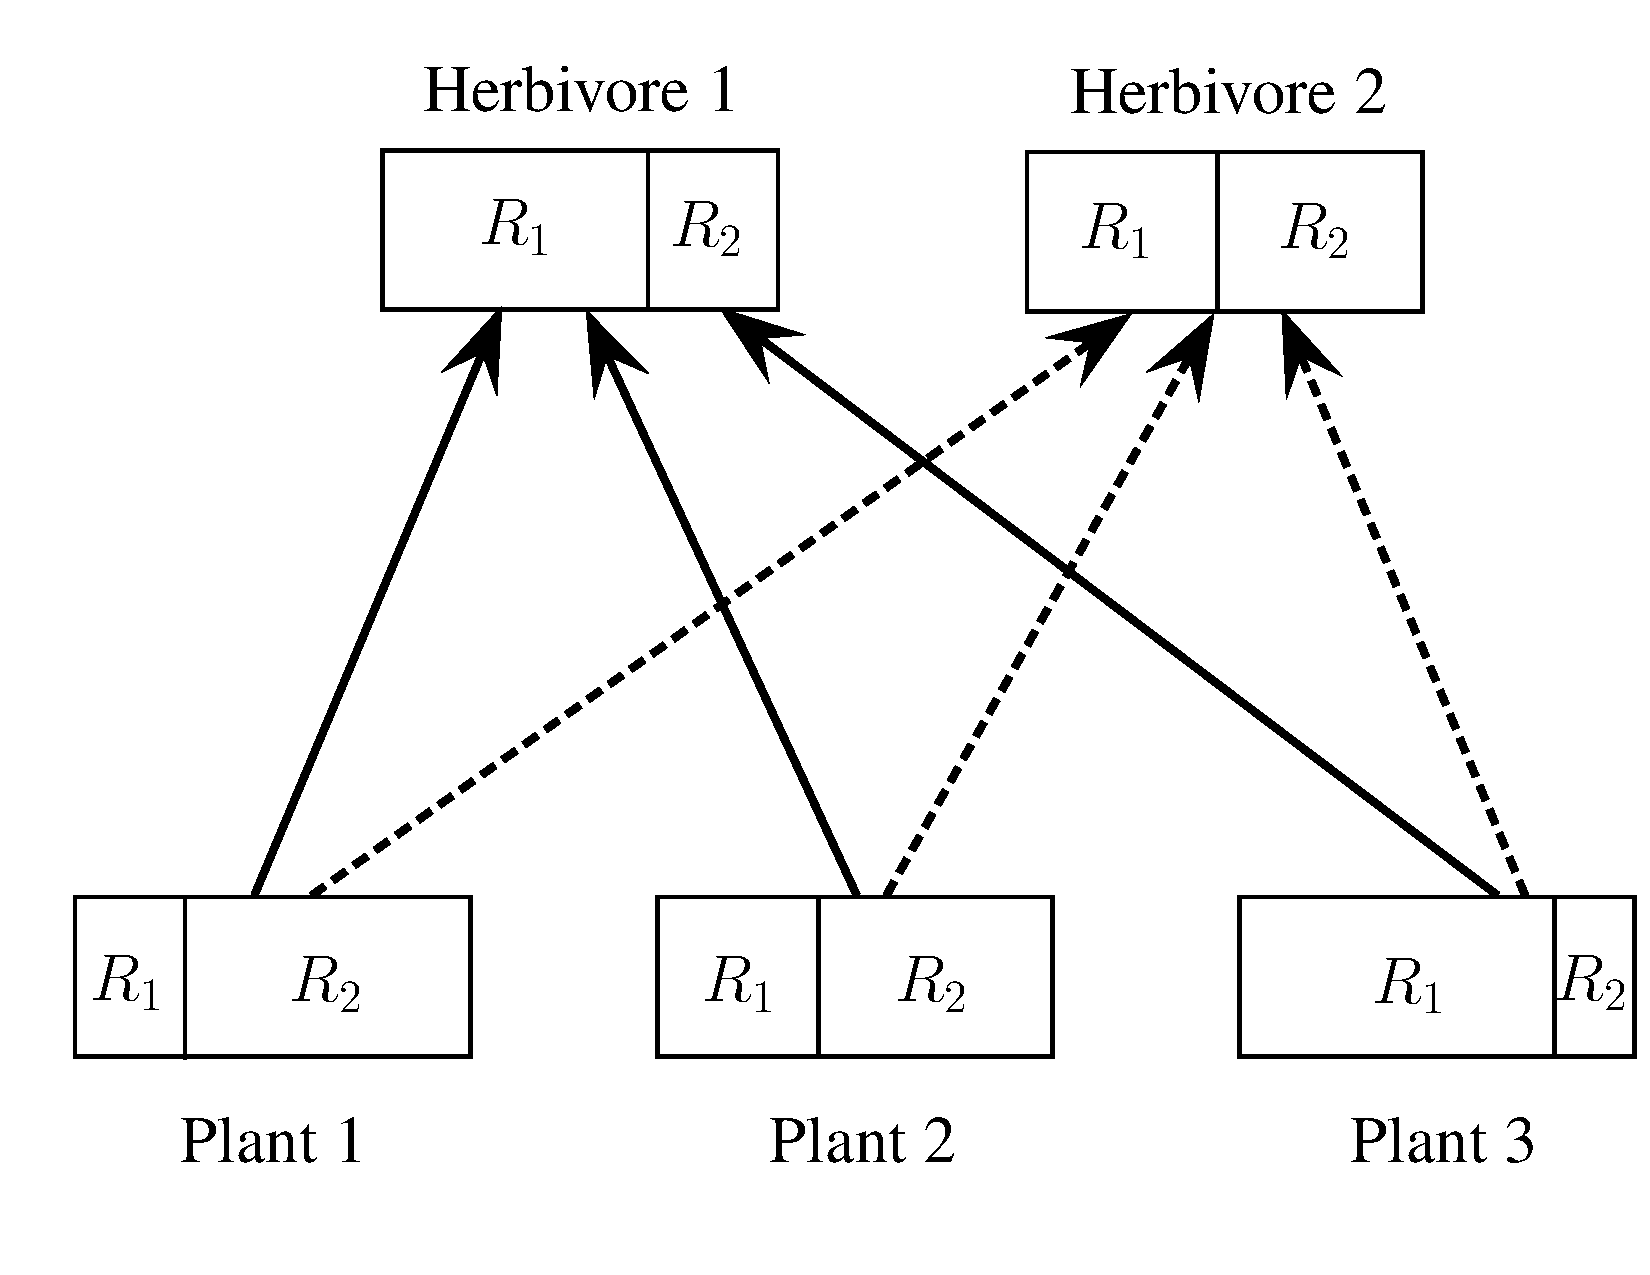
\includegraphics[width=12 cm, keepaspectratio, angle=-90]{Conceptuel} %angle=-90
\caption{Each herbivore species has its own resource ratio between resource 1 ($R_1$) and resource 2 ($R_2$). This species feeds on different plant species with different resource ratios. Herbivore requirements as well as their resource consumptions are key factors for their persistence.}
\label{conceptualfigure}
\end{figure}

\begin{figure}[h]
\centering
\includegraphics[width=14cm,keepaspectratio]{1plant} 
\caption{Phase plan with two herbivore species feeding on one plant species. Black lines are herbivore 1 ZNGI, dotted lines are herbivore 2 ZNGI, and grey arrow is the common consumption vector. Interpretations are quite similar with those from Tilman's model \citep{Tilman1982}. Roman numbers represent different zones for supply point position. Zone I and zone V do not provide sufficient amounts in $R_1$ and $R_2$ respectively. None herbivore species can live in these conditions. Zone II contains enough quantities of $R_1$ for herbivore 1, but not for herbivore 2. Zone III potentially has enough quantities of both resources for both herbivore species. In zone IV, only herbivore 2 can survive because there is not enough $R_2$ for herbivore 1. Supply point represents total amount of resources due to plant biomass rebuilding. Both herbivore species sample resources through the same consumption vector. In this exemple, the trajectory cross herbivore 2 ZNGY first and then herbivore 1 ZNGI. The crossing point with herbivore 1 ZNGI becomes an equilibrium point (E). Herbivore 1 is limited by $R_2$. Herbivore 2 is excluded.}
\label{herbifig}
\end{figure}

\begin{figure}[h]
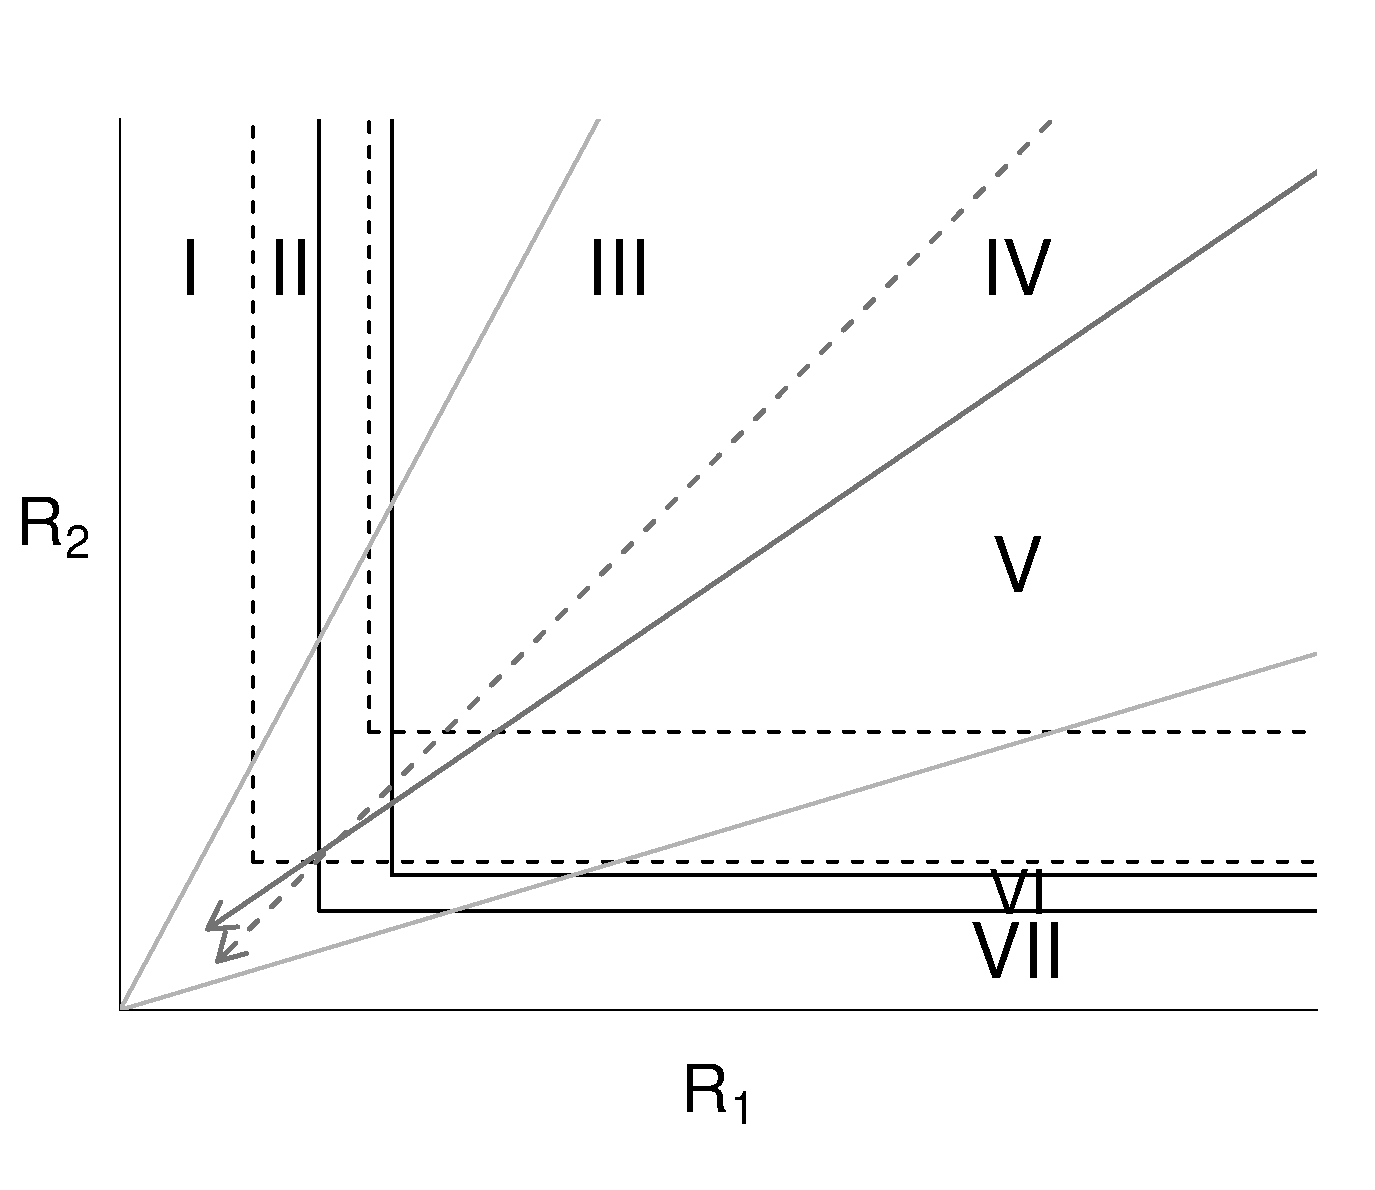
\includegraphics[width=15 cm, keepaspectratio]{Coexistence}
\caption{Phase plan for two coexisting herbivores. Lines represent boundary ZNGI, arrows are boundary vectors, and grey lines bound feasible supply conditions according to plants considered (i.e., feasibility cone). Continuous ZNGI and vector belong to herbivore 1, and dotted ZNGI and vector belong to herbivore 2. Zone I and zone VII contain not enough $R_1$ and $R_2$ respectively. Neither herbivore 1 nor herbivore 2 can survive. Zone II contains not enough $R_1$ for herbivore 2. Zone III does not allow herbivore 2 to survive if herbivore 1 is present. Zone V does not allow herbivore 1 to survive if herbivore 2 is present. Zone VI contains not enough $R_2$ for herbivore 1. If the supply point is within zone IV both herbivore can survive together: it is coexistence. Then, the cross zone of the two ZNGIs is a stable equilibrium point (SE).
}
\label{Coexistence}
\end{figure}

\begin{figure}[h]
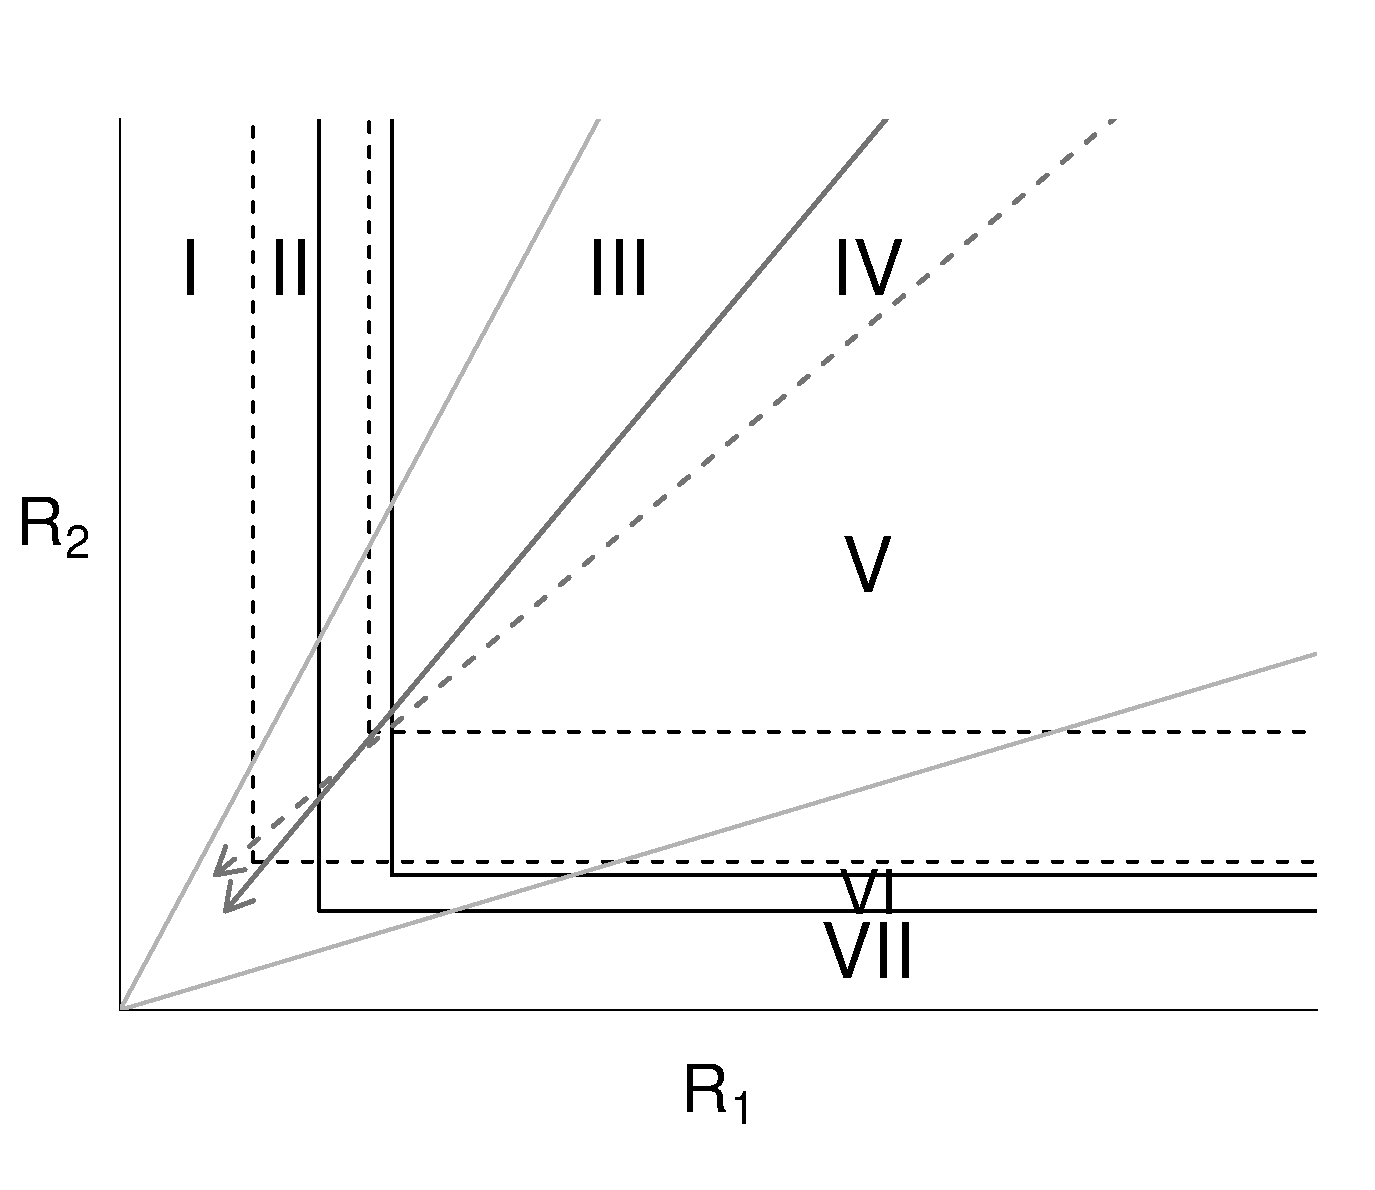
\includegraphics[width=15 cm, keepaspectratio]{Exclusion}
\caption{Phase plan for competitive exclusion. Representation of ZNGI and vectors is similar to figure \ref{Coexistence}, except for zone IV. This zone generally leads to exclusion of herbivore 1 or 2. The crossing zone of ZNGIs either can be a non stable equilibrium  (NSE) or does not allow coexistence of the two herbivore species. }
\label{Exclusion}
\end{figure}

\end{document}